\documentclass{article}

\usepackage{amsmath}
\usepackage[dvipdfmx]{graphicx}
\usepackage{caption}

\begin{document}
First, each methods used is described in section \ref{sec:methods},
and the results of experiments with each methods,
as well as the results of experiments using combinations of these methods,
are discussed in section \ref{sec:experiments}.

\section{Methods} \label{sec:methods}
    \subsection{Image processing}
        \subsubsection{Edge detection}
            Edge detection could be used to detect ice leads.

            Canny edge detection \cite{edge} is a popular edge detection algorithm.
            It consists of 4 steps:
            \begin{enumerate}
                \item Noise reduction
                \item Calculate image gradient
                \item Detect edges
                \item Sanitize edges
            \end{enumerate}

            \paragraph{Noise reduction}
                First, the image is smoothed using a Gaussian filter.
                This removes the noise from the image,
                which may affect the noise detection.

            \paragraph{Calculate image gradient}
                Next, the image is filetered in both horizontal and vertical direction
                with a Sobel kernel to obtain its first derivative.
                Then, gradient and its direction can be calculated as follows
                where $G_x$ and $G_y$ are the first derivative of horizontal
                and vertical direction respectively:

                \begin{eqnarray*}
                    \mathrm{Gradient} &=& \sqrt{G_x^2 + G_y^2} \\
                    \mathrm{Direction} &=& \arctan{\frac{G_y}{G_x}}
                \end{eqnarray*}

                The direction is rounded to one of the four directions
                we can handle on an image for the next step.

            \paragraph{Detect edges}
                An ``edge'' can be defined as a collection of pixels
                whose gradient is local maximum.
                Thus, given a pixel, compare its gradient with two adjacent
                pixels in the gradient direction,
                and if the pixel has the largest gradient,
                it can be said that the pixel constitutes an edge.
                By applying this calculation to all pixels,
                we obtain a binary image with ``edges''.

            \paragraph{Sanitize edges}
                Given two thresholds $t_\mathrm{max}$ and $t_\mathrm{min}$
                $(t_\mathrm{max} > t_\mathrm{min})$,
                an edge can be judged if it is a ``sure'' edge or not.
                At a pixel constituting an edge,
                if the gradient is above $t_\mathrm{max}$,
                then the pixel is determined as a ``sure'' edge.
                Conversely, if the gradient is below $t_\mathrm{min}$,
                the pixel will be discarded.
                For pixels whose its gradient is between two thresholds,
                the pixel can be said as a ``sure'' edge if it is connected to
                a ``sure'' edge, and if it's not, it will be also discarded.

        \subsubsection{Blur detection}
            Since satellite images contain a certain amount of clouds and its shadow,
            blur detection could be used to remove them as a preprocessing.

            Using Laplacian kernel and calculating its variance,
            an image can be determined if it is blurred or not \cite{blur}.
            The Laplacian kernel is expressed as follow:
            \begin{equation*}
                \begin{pmatrix}
                    0 & 1 & 0  \\
                    1 & -4 & 1 \\
                    0 & 1 & 0
                \end{pmatrix}
            \end{equation*}
            The kernel highlights rapid intensity changes,
            thus if its variance is small than given threshold,
            it means the image contains less intensity changes,
            which means it is ``blurry''.

            This calculation is applied to subdivided regions of the original image
            and if the region is ``blurry'',
            the region is determined to contain cloud (or shadow).

    \subsection{Unsupervised methods}
        \subsubsection{K-means clustering}
            K-means clustering \cite{kmeans} is a popular clustering algorithm.
            The goal is to classify all given data into $K$ clusters.
            The algorithm can be written as follows:
            \begin{enumerate}
                \item Assign each data to random cluster.
                \item Calculate center of each cluster.
                \item Reassign each data to the cluster with the closest center.
                \item Repeat 2 and 3 until the convergence.
            \end{enumerate}

        \subsubsection{Random forest classifier}
            Random forest classifier \cite{random} is a ensemble clustering algorithm.
            It consists of decision trees each trained on subdivided data.
            The idea here is to take average of a certain number of decision trees
            over-trained in diferent data respectively.

        \subsubsection{Autoencoder}
            An important aspect of data classification is
            the extraction of their features.
            An autoencoder \cite{autoencoder} is often used to extract features.
            It consists of an encoder and a decoder,
            which the encoder is trained to extract features as its output,
            and the decoder is trained to reconstruct the input from the output of the encoder.

            By training the autoencoder to reduce the difference between the input and output,
            it can be said that the output of the encoder is the features necessary to reconstruct the original input.

    \subsection{Semi-supervised methods}
        \subsubsection{Label spreading}
            Label spreading \cite{label} is semi-supervised classifying algorithm.
            Given data with labels and without labels,
            the goal is to label all unlabelled data based on the labelled data.

            For a given data, the algorithm constructs a
            fully connected graph with each datum as nodes,
            and the similarity between data as edges.
            Then, the labels are spread to all unlabelled nodes from labelled nodes.
            Additionally, the algorithm has a parameter
            $\alpha \in (0, 1)$, which indicates the uncertainty of given labels.
            The algorithm replaces the label of labelled data
            with probability $\alpha$ while spreading the label.

\section{Experiments} \label{sec:experiments}
    \subsection{Dataset}
        In the experiments described later,
        $1\times 1$ and $3\times 3$ pixels cropped from the original image
        are used as data.
        Since the original image has 21 channels,
        the data shape is $1\times 1\times 21$ or $3\times 3\times 21$.
        As training and validating data,
        $1\times 1$ and $3\times 3$ data labelled as whether
        the pixel (for $3\times 3$ datum, its center pixel)
        is a lead or not, are used.

        As an important fact, as shown later,
        the accuracy of a model for validating data does not
        directly represent its usefulness.
        The reason for this is thought to be the difference of their
        probability space between labelled data and (unlabelled) image data,
        which the former is not collected from an whole labelled image,
        but the labels are assigned to the pixels extracted from unlabelled image.

    \subsection{Prior experiment} \label{sec:vit}
        Using labelled dataset,
        supervised training has done to a model based on Vision Transformer \cite{vit}.
        It performed accuracy of 0.8395, and its rollout is shown in Figure \ref{fig:rollouts}.
        Although the accuracy inferior to other methods as shown later,
        this method is likely the most effective when looking at rollout.

    \subsection{Edge detection} \label{sec:edge}
        As two thresholds, $(t_\mathrm{max}, t_\mathrm{min}) = (0, 96)$ is used.
        The result is shown in Figure \ref{fig:rollouts}.
        We can see that the result is similar to the rollout of prior experiment.

    \subsection{Blur detection}
        Images are subdivided into $128 \times 128$ pixels,
        and the variance of the Laplacian is calculated for each region.
        The original image and result are shown in Figure \ref{fig:blur}.

        We can see that regions with clouds are determined blurry,
        but especially in the bottom image,
        region with lead also has a certain value of the variance,
        which leads the conclusion that the method is severe to be used for cloud removal.

        \begin{figure}
            \centering
            \begin{minipage}{0.49\hsize}
                \centering
                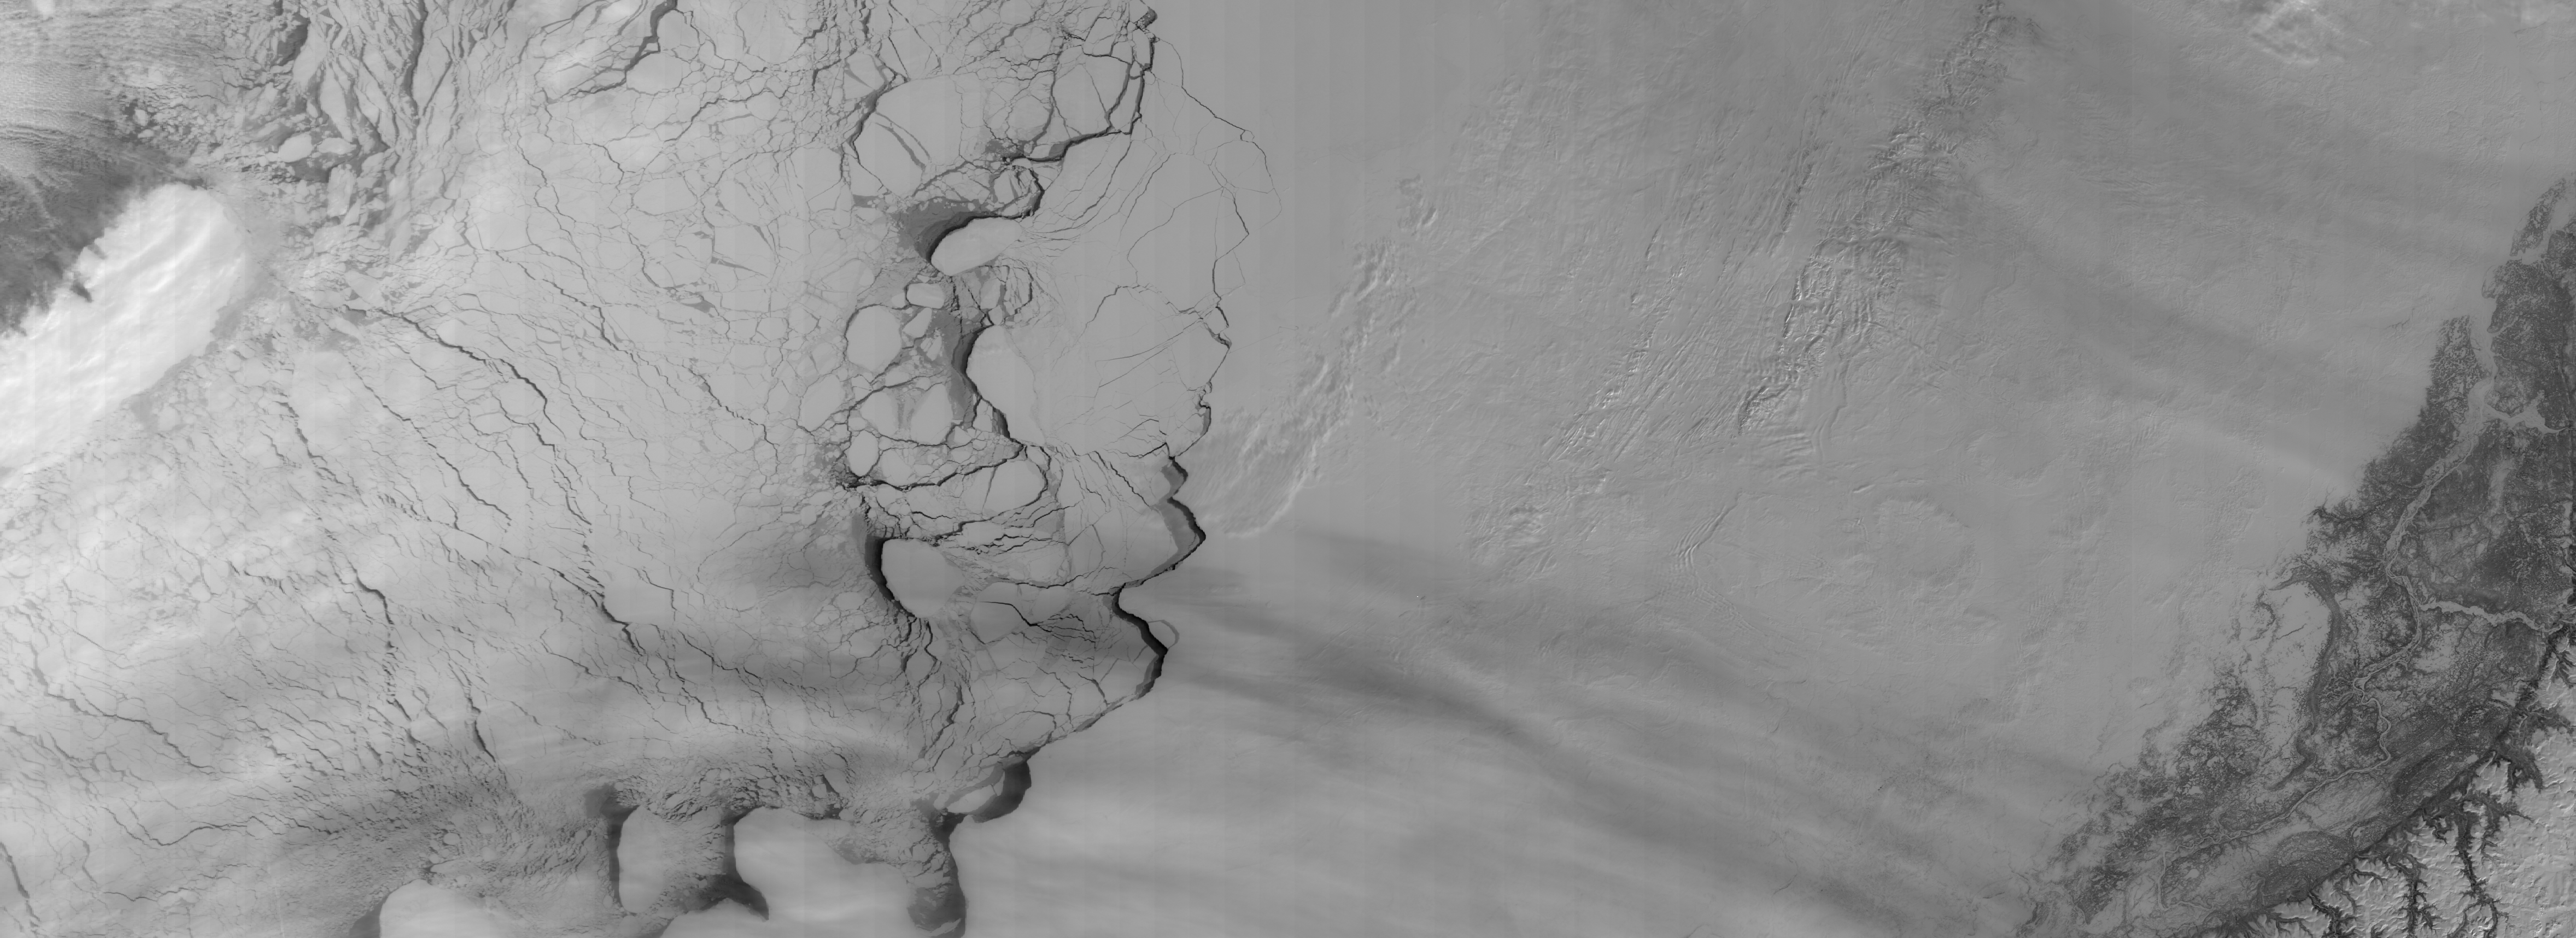
\includegraphics[width = 1\hsize]{1.png}
                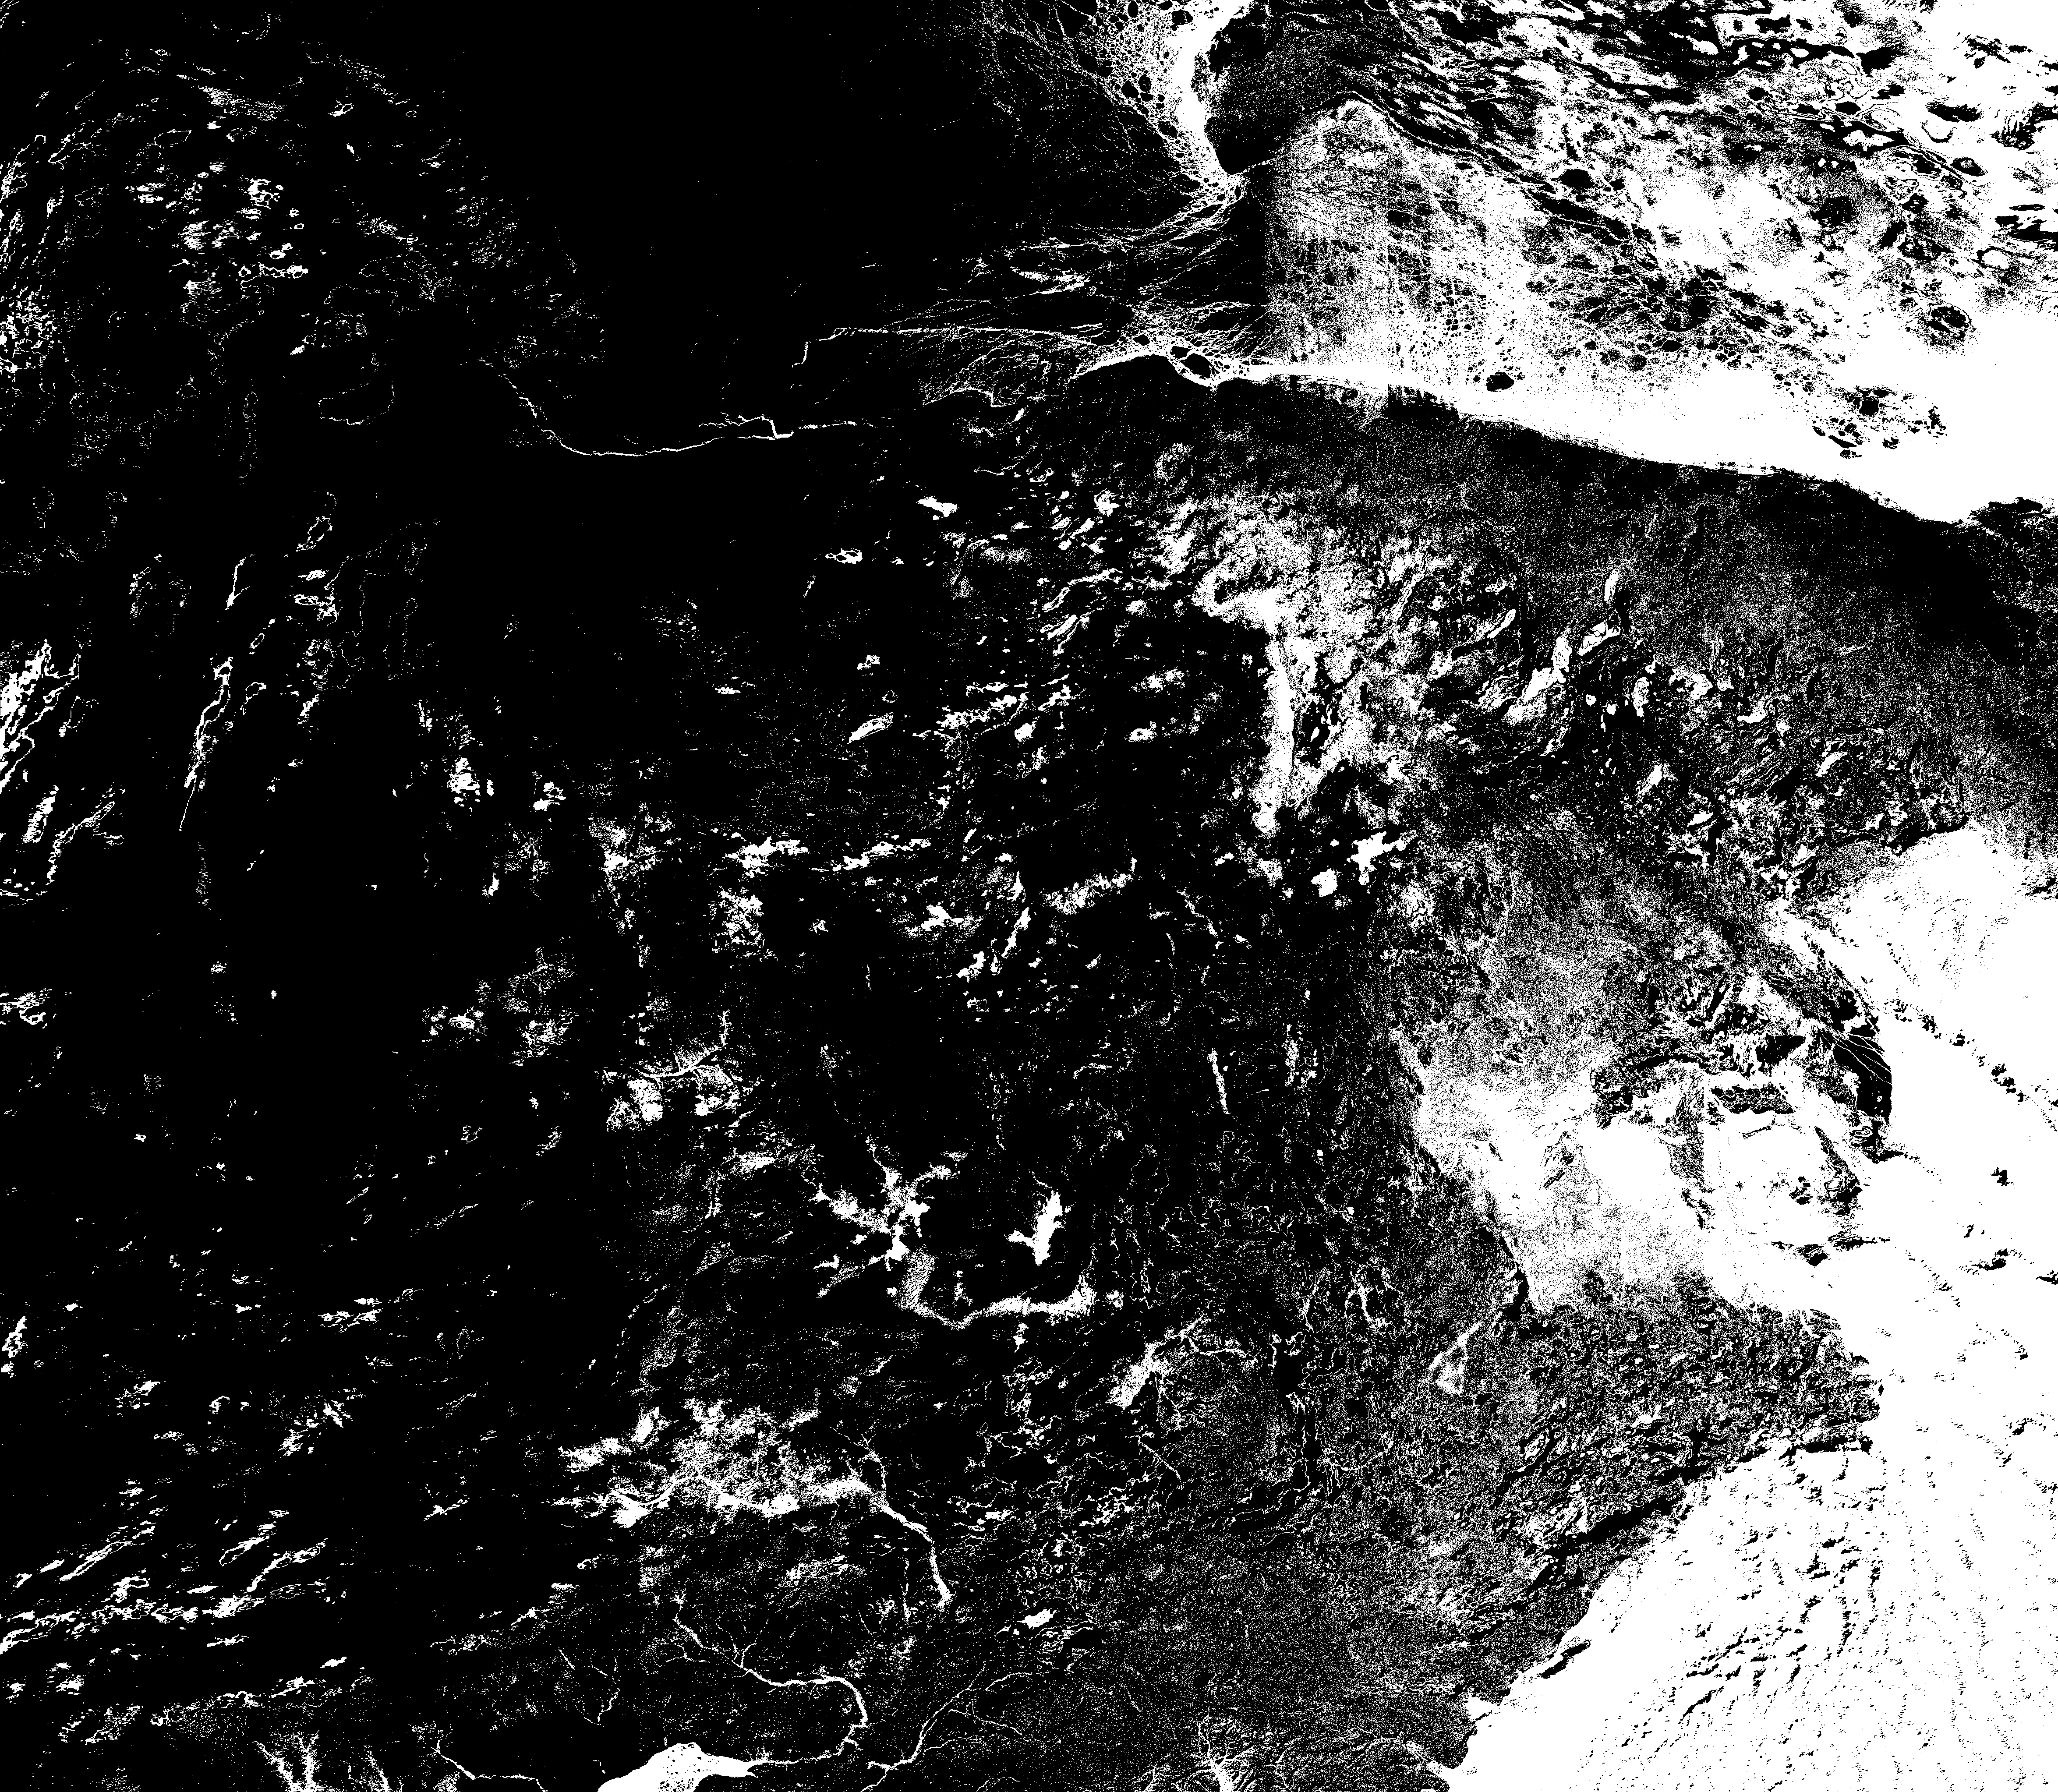
\includegraphics[width = 1\hsize]{2.png}
                \caption*{(a)}
            \end{minipage}
            \begin{minipage}{0.49\hsize}
                \centering
                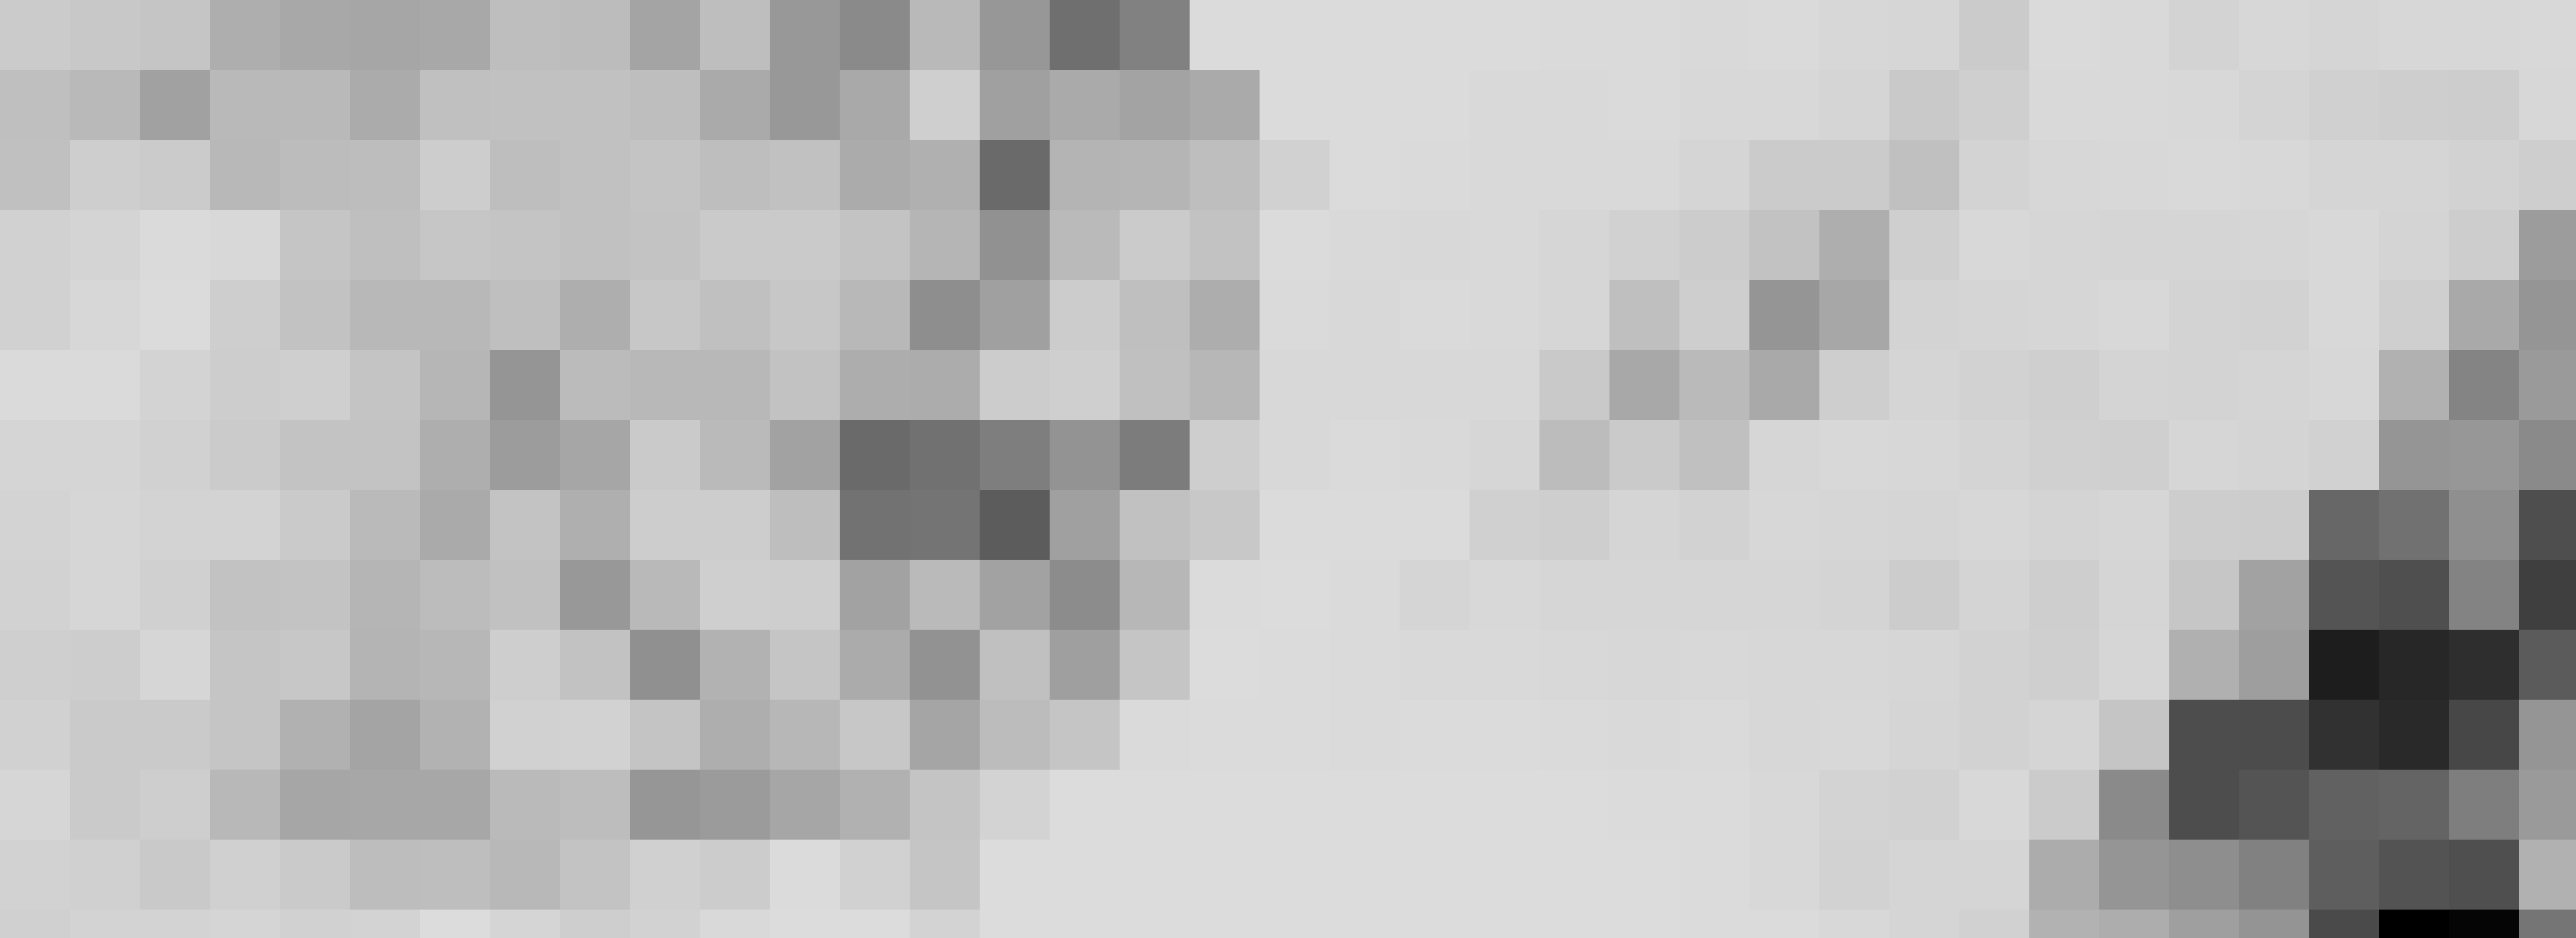
\includegraphics[width = 1\hsize]{1_blur.png}
                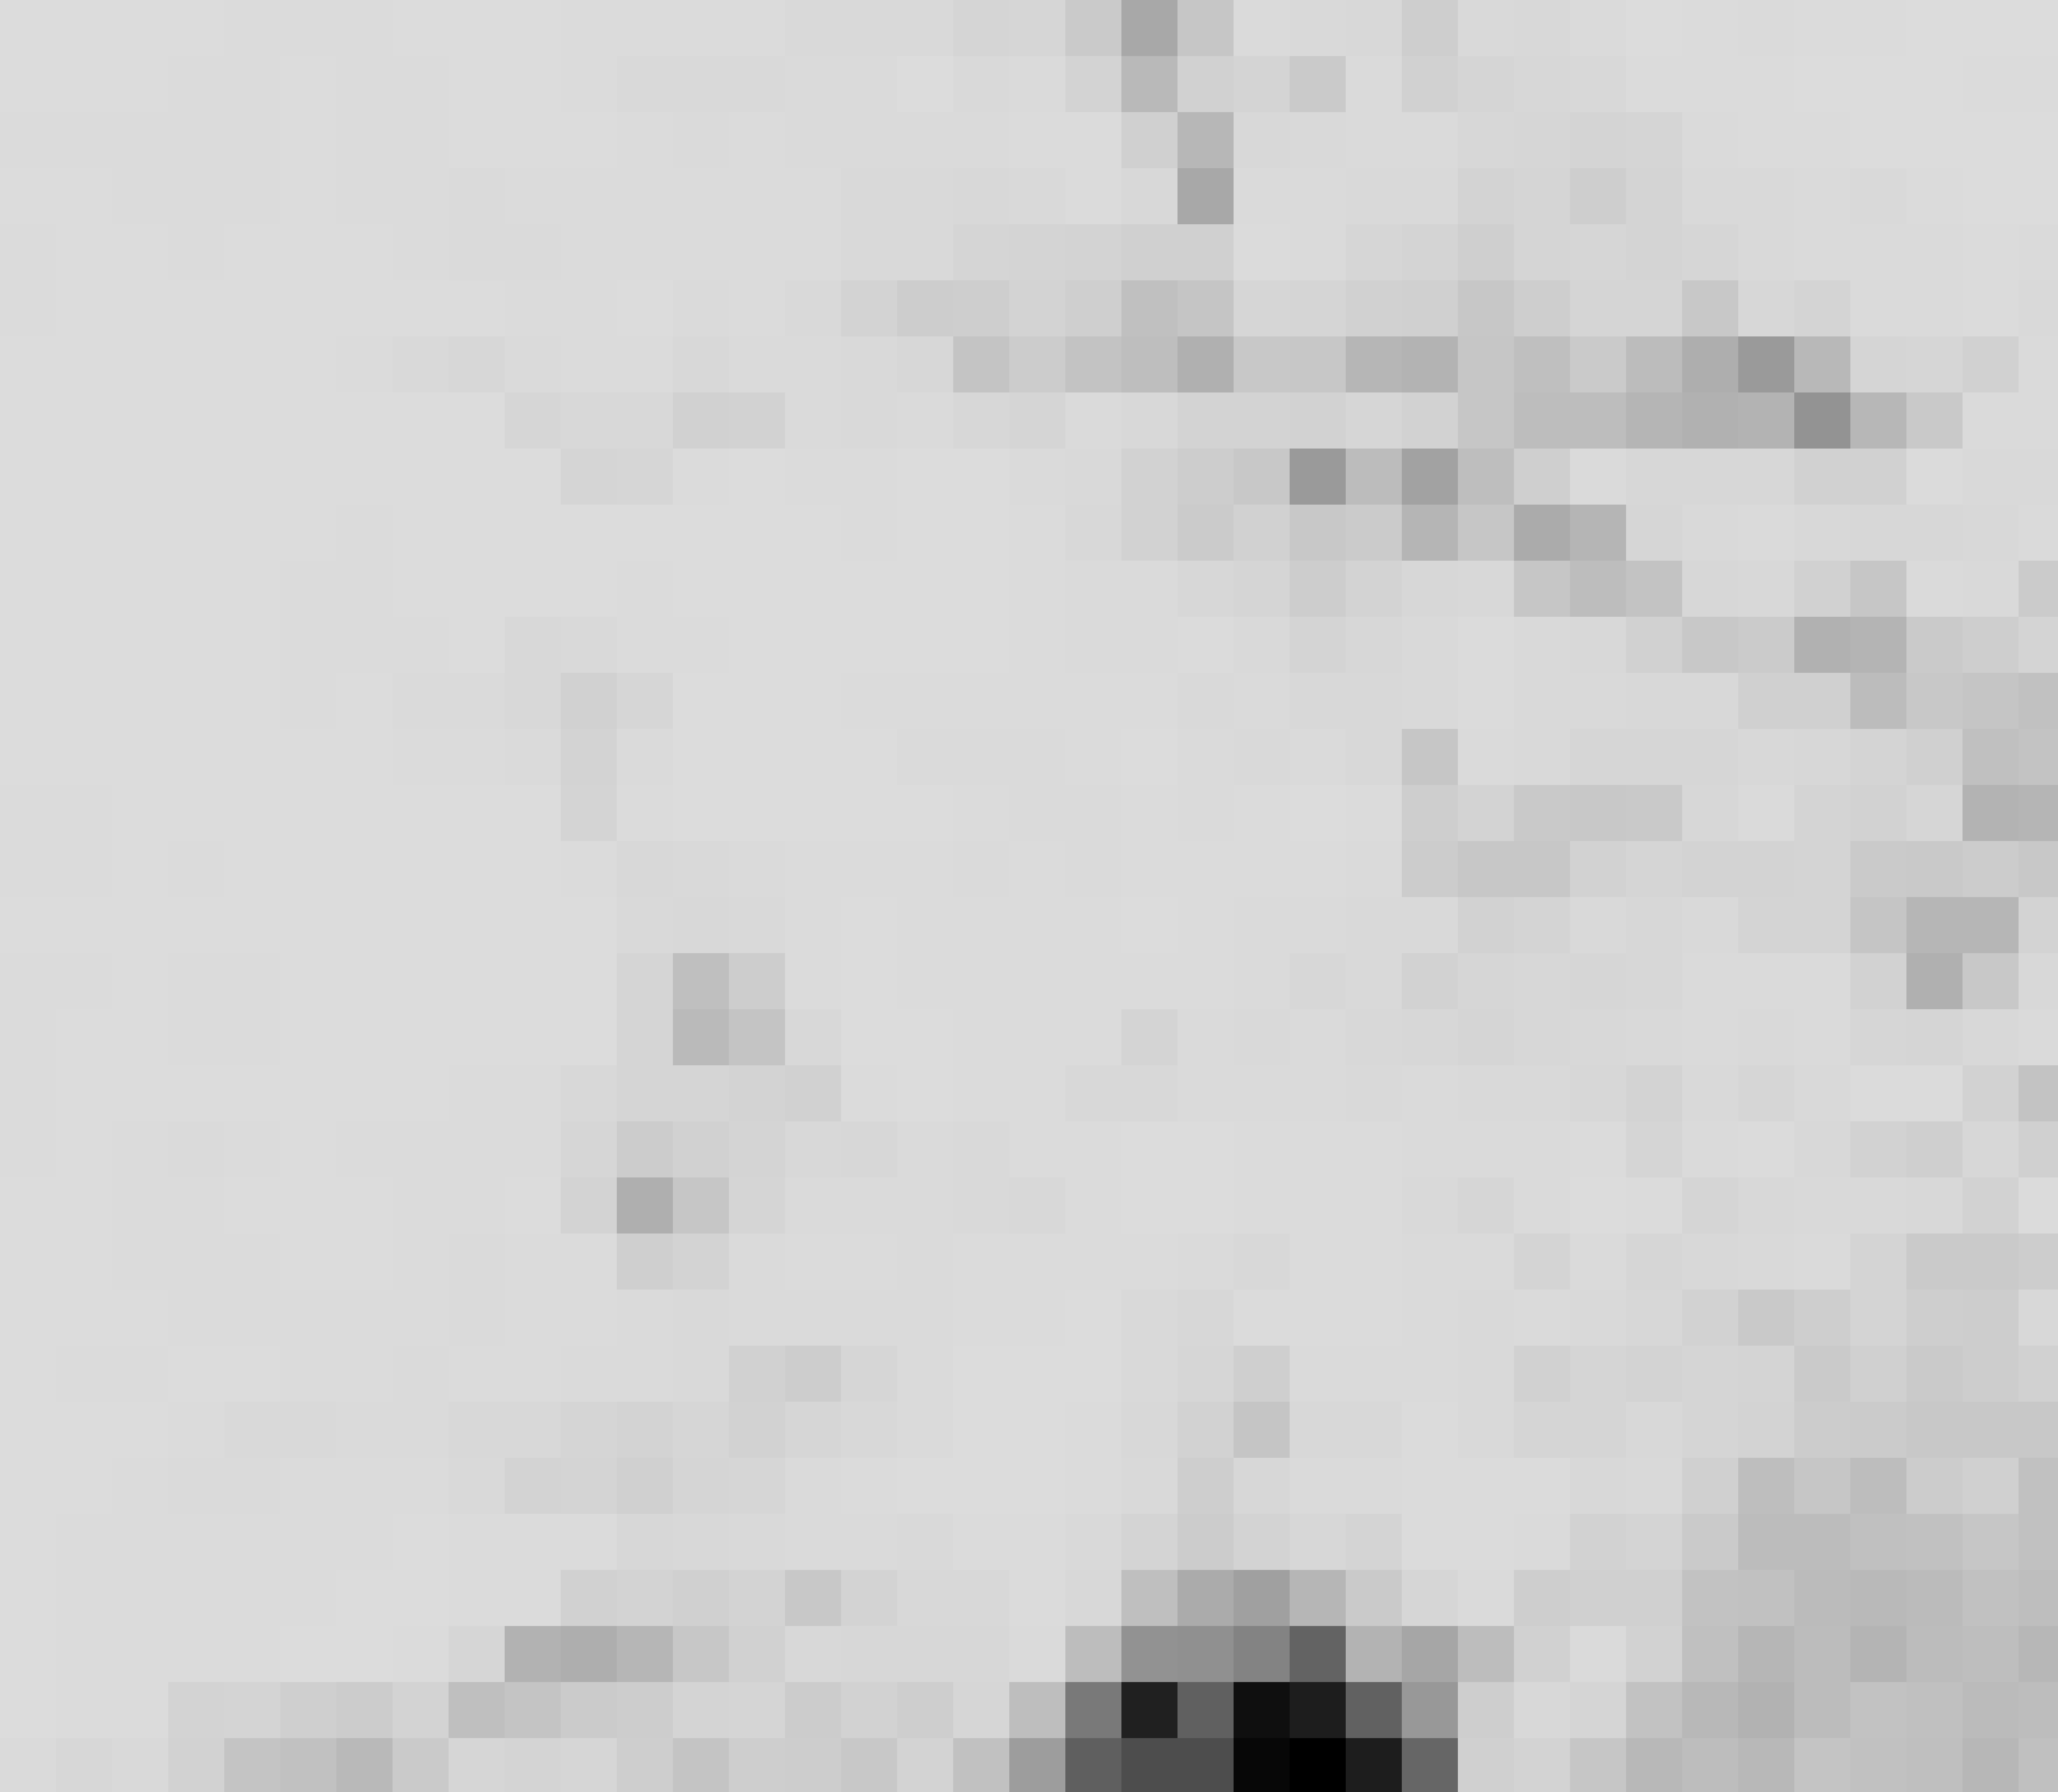
\includegraphics[width = 1\hsize]{2_blur.png}
                \caption*{(b)}
            \end{minipage}
            \caption{
                Blur detection results.
                (a) Channel 1 of the original image.
                (b) Variance of the Laplacian by region.
                The brighter the region, the more blurred it is.
            }
            \label{fig:blur}
        \end{figure}

    \subsection{K-means clustering} \label{sec:kmeans}
        K-means clustering with $K = 8$ is done with sampled data
        both $1\times 1$ and $3\times 3$ size.
        Considering the 2 ``darkest'' clusters as the lead,
        the model performed accuracy of 0.7498 training with $1\times 1$ data,
        and 0.7893 with $3\times 3$ data.
        The rollouts of model trained with $3\times 3$ data
        are shown in Figure \ref{fig:rollouts}.

    \subsection{Label spreading} \label{sec:label}
        \subsubsection{Using raw data}
            Label spreading is done with sampled $1\times 1$ data.
            The model performed accuracy of 0.7127.

        \subsubsection{Using autoencoder}
            Since the data has 21 channels,
            which may be too large to classify,
            an autoencoder is trained to extract features,
            and apply label spreading with the features.
            The model performed accuracy of 0.8321 with $1\times 1$ data,
            and 0.8943 with $3\times 3$ data.
            The rollouts of model trained with $3\times 3$ data
            are shown in Figure \ref{fig:rollouts}.

    \subsection{Random forest} \label{sec:random}
        Random forest classifier with 20 ensembles is trained with
        both $1\times 1$ and $3\times 3$ size data.
        The model performed accuracy of 0.9244 trained with $1\times 1$ data,
        and 0.9478 with $3\times 3$ data.
        We considered using features gained from autoencoder just as
        we did when using the label spreading method,
        but no improvement was seen.
        The rollouts of model trained with $3\times 3$ data
        are shown in Figure \ref{fig:rollouts}

    \begin{figure}
        \centering
        \includegraphics[width = 1\hsize]{rollouts1.png}
        \includegraphics[width = 1\hsize]{rollouts2.png}
        \caption{
            Rollouts of each model to two images.
            The upper left figure is channel 1 of the original image,
            and rollout of Vision Transformer (Section \ref{sec:vit})
            and edge detection (Section \ref{sec:edge}).
            Rollout of K-means clustering (Section \ref{sec:kmeans}),
            label spreading (Section \ref{sec:label}),
            and random forest (Section \ref{sec:random})
            from left to right in the bottom row.
            Accuracy of the model are shown in Table \ref{tab:accuracy}
        }
        \label{fig:rollouts}
    \end{figure}

    \begin{table}
        \centering
        \caption{Accuracy of models}
        \label{tab:accuracy}
        \begin{tabular}{l|cc} \hline
            & $1\times 1$ data & $3\times 3$ data \\ \hline
            Vision Transformer & - & 0.8395 \\
            K-means & 0.7498 & 0.7893 \\
            Label spreading & 0.8321 & 0.8943 \\
            Random forest & 0.9244 & 0.9478 \\ \hline
        \end{tabular}
    \end{table}

\begin{thebibliography}{99}
    \bibitem{edge}{
        J. Canny,
        ``A Computational Approach to Edge Detection'',
        IEEE Transactions on Pattern Analysis and Machine Intelligence,
        1986
    }

    \bibitem{blur}{
        R. Bansal, G. Raj and T. Choudhury,
        ``Blur image detection using Laplacian operator and Open-CV'',
        International Conference System Modeling \& Advancement in Research Trends,
        2016
    }

    \bibitem{kmeans}{
        G. Ball and D. Hall,
        ``ISODATA, a Novel Method of Data Analysis and Pattern Classification'',
        Stanford Research Institute,
        1965
    }

    \bibitem{random}{
        L. Breiman,
        ``Random Forests'',
        Machine Learning,
        2001
    }

    \bibitem{autoencoder}{
        M. Kramer,
        ``Nonlinear principal component analysis using autoassociative neural networks'',
        AIChE Journal,
        1991
    }

    \bibitem{label}{
        D. Zhou, O. Bousquet, T. Lal, J. Weston and B. Schoelkopf,
        ``Learning with local and global consistency'',
        Advances in Neural Information Processing Systems,
        2004
    }

    \bibitem{vit}{
        A. Dosovitskiy, L. Beyer, A. Kolesnikov, D. Weissenborn, X. Zhai, T. Unterthiner, M. Dehghani, M. Minderer, G. Heigold, S. Gelly, J. Uszkoreit and N. Houlsby,
        ``An Image is Worth 16x16 Words: Transformers for Image Recognition at Scale'',
        International Conference on Learning Representations,
        2021
    }
\end{thebibliography}
\end{document}